\documentclass[a4paper,twoside]{article}

\usepackage{epsfig}
\usepackage{amssymb}
\usepackage{amstext}
\usepackage{amsmath}
\usepackage{amsthm}
\usepackage{multicol}
\usepackage{pslatex}
\usepackage{apalike}
\usepackage{SCITEPRESS}


\usepackage{listings}
\usepackage{xcolor}
\usepackage{subfig}
\usepackage{graphicx}
\usepackage{epstopdf}
\usepackage{flushend}
\usepackage{listings}
\usepackage{color}
\usepackage{multicol}
\usepackage{amsmath}


\usepackage{floatrow}

\colorlet{punct}{red!60!black}
\definecolor{background}{HTML}{EEEEEE}
\definecolor{delim}{RGB}{20,105,176}
\colorlet{numb}{magenta!60!black}

\lstdefinelanguage{json}{
    basicstyle=\scriptsize\ttfamily,
    numbers=none,
    numberstyle=\scriptsize,
    stepnumber=1,
    numbersep=8pt,
    showstringspaces=false,
    breaklines=true,
    frame=none,
    backgroundcolor=\color{background},
    literate=
     *{0}{{{\color{numb}0}}}{1}
      {1}{{{\color{numb}1}}}{1}
      {2}{{{\color{numb}2}}}{1}
      {3}{{{\color{numb}3}}}{1}
      {4}{{{\color{numb}4}}}{1}
      {5}{{{\color{numb}5}}}{1}
      {6}{{{\color{numb}6}}}{1}
      {7}{{{\color{numb}7}}}{1}
      {8}{{{\color{numb}8}}}{1}
      {9}{{{\color{numb}9}}}{1}
      {:}{{{\color{punct}{:}}}}{1}
      {,}{{{\color{punct}{,}}}}{1}
      {\{}{{{\color{delim}{\{}}}}{1}
      {\}}{{{\color{delim}{\}}}}}{1}
      {[}{{{\color{delim}{[}}}}{1}
      {]}{{{\color{delim}{]}}}}{1},
}


\lstset{breaklines=true}

\begin{document}

\title{MoBio\subtitle{A mobile system for collecting data from sensors} }

\author{\authorname{Petr Je\v{z}ek\sup{1} and Roman Mou\v{c}ek\sup{1}}
\affiliation{\sup{1}New Technologies for the Information Society, 
              Department of Computer Science and Engineering,
              Faculty of Applied Sciences,
              University of  West Bohemia,
              Univerzitn\'{i} 8,
              306 14  Plze\v{n},
              Czech Republic}
\email{jezekp@ntis.zcu.cz, moucek@kiv.zcu.cz}
}   

\keywords{MoBio, Sensor, Android system, Mobille application, Terminology, Data transfer}

\abstract{There are a lot of sensors on the market for monitoring of human health or a fitness level. Sensors enable collection of data from human body and their displaying to the user. Advanced devices also enable data transfer to remote servers where they are processed. These sensors use different topology  and data format for data transfer. It makes them difficult to be integrated with neuroinformatics databases raising within the community. As a solution a terminology describing data from limited collection of sensors is presented. This terminology si implemented  in the odML format and integrated in a proof-of-concept Android application. This application enables collection of data from basic set of sensors. The data transfer, their storage and visualization in a remote neuroinformatics database EEGBase is also presented.}

\onecolumn \maketitle \normalsize \vfill

\section{\uppercase{Introduction}}
\label{sec:introduction}

\noindent 
There are a lot of factors affecting human health. Factors such as genetics, environmental influence or internal state of an individual cannot be easy measured. On the other hand there are factors as blood pressure, glucose level or heart rate that can be measured relatively easy, non-invasively by cheap sensors. For a long time electrophysiological experiments have been conducted in laboratories equipped by common desktop computers and non-transferable measuring devices. Fortunately situation is rapidly changing in these days. The one of reasons is increasing popularity of smart devices such as phones or tablets. According to eMarketer \cite{emark} two billions of people will own a smart-phone in 2016. Simultaneously a lot of relatively cheap sensors for measurement of potentials from the human body is available on the market. These sensors often transfer data wirelessly, they can be read and processed by smart devices. This technical progress enables a particular shift of treatment from hospitals to home environments and facilitates collecting of data during outdoor activities. The obtained data can be used by two fundamental intersecting ways. 

The first assistive technology approach serves to stimulating, maintaining or improving functional capabilities of people with special needs including disabled people or aging population. Getting independence and self-sufficiency increases quality of life in general. 

The second approach is focused on sportsmen or actively living people. Measurements are based on a monitoring of persons when they are performing specific activities (e. g. running or long distance walking). The data are used for a long term monitoring of the fitness level. 

The existing sensors usually store data in proprietary formats. These data are transfered to closed databases. It makes them difficult to be used in experimental laboratories. 

We operate a completely equipped laboratory \cite{10.3389/fninf.2014.00020} for electrophysiological measurements. We are focused  mainly on Electroencephalography (EEG) and Event-related potentials (ERP). Except of the fixed laboratory we also operate a mobile laboratory equipped by a set of laptops and portable measuring devices for performing experiments out of the laboratory. With advancing efforts for extension the laboratory to collect broader spectrum of data (e. g. blood pressure, Electrocardiogram (EKG), glucose level, heart rate) we are extending our infrastructure (hardware devices and software tools) to support  measurements of heterogeneous data from various kind of sensors.  In this paper we are proposing a terminology describing data coming from health sensors and  a prototype of mobile client for collecting data from these sensors. The client provides integration with a limited set of devices and enables data transfer and visualization in a remote storage.

\section{\uppercase{state of the art}}
\label{sec:state-of-the-art}

\noindent
According to \cite{Lowe2012242} applications using sensors can be divided into three categories. The first category Smart Phone Applications use either GPS or the
on-board kinematic sensors as the technologies of choice for monitoring exercise. The second category comprises of any system that uses a central controller
and an external sensor. The last category comes from image processing domain. It uses a combination of a computer screen and a camera. The camera monitors the exact movement and position of the entire body during exercise. The screen is used for the interaction with the user.

The first category represents application such as Endomondo or Runkeeper. The second category Nike+, miCoach, Garmin Heart Belt or Fora Active tonometer. The typical representative of third category is Microsoft Kinect.

While Microsoft Kinect is designed for the indoor use all other devices are designed mostly for the outdoor use. 

Available tools and sensors are usually designed for one specific activity. They are able to record only limited variety of data. In addition, due to proprietary structure they do not provide variability for integration with other systems. 

Moreower, neuroinformatics community identified problems with a long-term description, storage and management of experimental data/metadata \cite{CRCNS}. Ontology for Experimental Neurophysiology (OEN) \cite{10.3389/conf.fninf.2014.18.00044} is a semantic web approach to describe terminology used in biomedical and neuro sciences. As a member of International Neuroinformatics Coordinating Facility (INCF) \cite{INCF} we are being developing a system for long term storage and management of EEG/ERP experiments - EEGBase \cite{ISI:000306821100004}. A mobile EEGBase client \cite{10.3389/conf.fninf.2013.09.00046} is a supplementary tool that enables collecting experiments out of the laboratory and provides an on-line synchronization with EEGBase.


\section{\uppercase{Topologies and Data Transfer}}
\label{topology_data_transfer}

\noindent 
Sensors use different way to manipulate data. Some sensors have own display or internal memory for storing measured data these data can be transfered later. These devices usually provide a complete history of stored measurements. On the other hand devices such as heart rate meters do not have internal memory. Data can be transfered only in time of measurement. According to way of data distribution we defined three levels of topologies.

\begin{itemize}
 \item one-layer - The sensor is a stand-alone unit with controls, display and memory. Such a sensor is completely controlled without any connections to a remote system.   
 \item two-layers - The sensor only measures the data that send to a remote system. This system can be a common computer/laptop or a smart phone/watch etc. 
 \item three-layers - This topology adds a cloud service to the two-layers topology. Data are send to the server where they are stored analyzed. 
\end{itemize}

There are a lot of sensors in one-layer topology including various glucometers, tonometers, stepcounters etc. These devices usually enables easy manipulation and do not require connection to any other system. Anyway the data are stored in a proprietary storage that do not provide means for communication with other systems. Some sensors including heart rate belts or some step counters do not have own display. For the data transfer are usually used technologies Bluetooth or ANT (resp ANT+)\footnote{ANT is a the protocol while ANT+ is a set of mutually agreed upon definitions for what the information sent over ANT represents.}. Data are usually displayed on a smart device screen. Because of limited performance of mobile devices only a basic data processing is provided. There is few exceptions as BlibCare tonometer equipped by WiFi. It enables a direct data transfer to a server using a home network. 



\begin{table*}[th!]
\centering
\caption{Tested Systems}
\label{tab:tested_systems}
\begin{tabular}{|l|c|c|c|c|c|c|c|}
\hline
               & \multicolumn{1}{l|}{\begin{tabular}[c]{@{}l@{}}Internal\\  sensors\end{tabular}} & \multicolumn{1}{l|}{\begin{tabular}[c]{@{}l@{}}External\\ sensors\end{tabular}} & \multicolumn{1}{l|}{\begin{tabular}[c]{@{}l@{}}Continuous\\  measurements\end{tabular}} & \multicolumn{1}{l|}{\begin{tabular}[c]{@{}l@{}}Single\\  measurements\end{tabular}} & \multicolumn{1}{l|}{Statistics} & \multicolumn{1}{l|}{\begin{tabular}[c]{@{}l@{}}Cloud\\ Service\end{tabular}} & \multicolumn{1}{l|}{Design} \\ \hline

Endomondo      & 2                                                                                & 3                                                                               & \textbullet                                                                                        &                                                                                     & \textbullet                                & \textbullet                                  & +                           \\ \hline
Runstatic      & 2                                                                                & 2                                                                               & \textbullet                                                                                        &                                                                                     & \textbullet                                & \textbullet                                 & +                           \\ \hline
Pedometer      & 1                                                                                &                                                                                 & \textbullet                                                                                        &                                                                                     & \textbullet                                & \textbullet                                  & -                           \\ \hline
Push-ups       & 1                                                                                &                                                                                 & \textbullet                                                                                        &                                                                                     & \textbullet                                & \textbullet                                  & +                           \\ \hline
Heart rate     & 1                                                                                &                                                                                 &                                                                                         & \textbullet                                                                                    & \textbullet                                & \textbullet                                  & +                           \\ \hline
Sport Tracker  & 1                                                                                & 2                                                                               & \textbullet                                                                                        &                                                                                     & \textbullet                                & \textbullet                                  & +                           \\ \hline
Health Tracker &                                                                                  &                                                                                 &                                                                                         &                                                                                     & \textbullet                                &                                   & -                           \\ \hline
Madbarz        &                                                                                  &                                                                                 &                                                                                         &                                                                                     & \textbullet                                & \textbullet                                  & +                           \\ \hline
eVito        & 1                                                                                 & 5                                                                                  & \textbullet  & \textbullet                                                                                      &  \textbullet                                                                                   & \textbullet                                                                & +                           \\ \hline
\end{tabular}
\end{table*}



\section{\uppercase{Tested systems}}
\label{tested_systems}
\noindent
From Sections \ref{sec:state-of-the-art} and \ref{mobile_app_prototype} we can observer that sensors based on the three layers topology are most suitable for long term storage and management of collected data. When these devices provide a remote transfer of data to a server these devices are suitable to be integrated with neuroinformatics databases. The biggest obstacle is a data format of transferred data. When devices implement Bluetooth or ANT+ technologies they can use a lot of defined profiles including e. g. BLP, CSCP, GLP, HRP, WSP\footnote{https://developer.bluetooth.org/TechnologyOverview/Pages/Profiles.aspx} for Bluetooth, or Weight Scale a Heart rate \footnote{https://www.thisisant.com/developer/ant-plus/device-profiles} for ANT+. Table \ref{tab:tested_systems} summarizes systems we tested. We selected these they provide at least a cloud service or statistics. For all systems we count number of supported internal sensors (e. g. smart phone GPS) and external sensors. We can observe that the support of sensors is very limited. Even the last two do not support any sensor, data are inserted manually. The last column \emph{Design} is more or less a subjective evaluation of the user interface. Although all tested systems use ANT or Bluetooth they implement a proprietary transfer format instead of using any available profile. 


\section{\uppercase{Mobile application prototype}}
\label{mobile_app_prototype}


\subsection{System Scope}

On the basis of difficulties with close-source dedicated devices we present a prototype of a mobile system that solves described problems by implementing a database relying on a standardized terminology describing sensors data. The mobile system ensures the outdoor usage or the usage in environments without the Internet connectivity. When the client gets on-line the stored data are synchronized with EEGBase. Such a system aggregates data from various sensors in one place. Moreover, the data stored in a flexible data storage on the server can be used by human reared or processed by automatic readers.

\subsection{Format Selection}

Existing data formats are based on different levels of abstraction from low-level binary formats, through highly abstract implementation-independent data formats to formats based on semantic web ontologies. We require a format that provides a sufficient level of abstraction to be system independent on one hand, but it should be easy-to-use without any specific requirements for user's knowledge on the other hand.

When the aim of the tool is to support large collections of sensors it must store data in a flexible data format. Moreover, we prefer open-source formats supported and accepted by large neuroscience community. So far, the working group entertains two approaches towards defining a standard, which may eventually be merged \cite{10.3389/conf.fninf.2013.09.00069}. The first one Hierarchical Data Format (HDF5) \cite{hdf5} or respectively epHDF that is specialized HDF5 for electrophysiology. The second one NIX \cite{Stoewer:2014}  provides a data model for storing experimental data in HDF5, together with metadata in the odML format \cite{10.3389/fninf.2011.00016}. Both formats are maintained by The INCF Task Forces on Electrophysiology\footnote{http://www.incf.org/programs/datasharing/electrophysiology-task-force}. The odML format brings the advantages of platform-independence and simplicity and human-readability. We selected odML as a suitable format for presented tool because it ensures a compatibility with other systems developed in neuroinformatics community.

\subsection{Implementation}

With regard to the use of open source technologies in maximal range we decided to implement the system for the Android platform. The main benefit of this selection is its availability on large collections of devices including both tablets and mobile phones. According to StatCounter\footnote{http://gs.statcounter.com} more then 60\% of devices are operated by Android.   Moreover, there is a lot of cheap devices on the market, large community of developers and publication of applications is easy. 

The presented proof of concept implementation provides basic functionality including management of user accounts,  support of a limited set of sensors, or visualization of stored data.

The registration form includes both basic information such as name or email and advanced information such as gender, weight, tallness, current fitness level etc. All these data are required because they can affect results of measurements.

The supported devices must enable either Bluetooth nor ANT transfer. In a current implementation we support limited set of devices produced by Garmin and Fora producers. When the device is paired then the user can transfer the data. Figure \ref{fig:mob_app_prev} shows a basic functionality provided to the logged user. Figure \ref{fig:capture_a} shows list with one paired device - Garmin Heart Rate Sensor. Current heart rate is in Figure \ref{fig:capture_b}. When the user starts a measurement data are continuously stored in the device and a chart is continuously plotted as shown in Figure \ref{fig:capture_c}.


\begin{figure*}
% Use the relevant command to insert your figure file.
% For example, with the graphicx package use
\begin{tabular}{c}
\subfloat[List of available sensors]{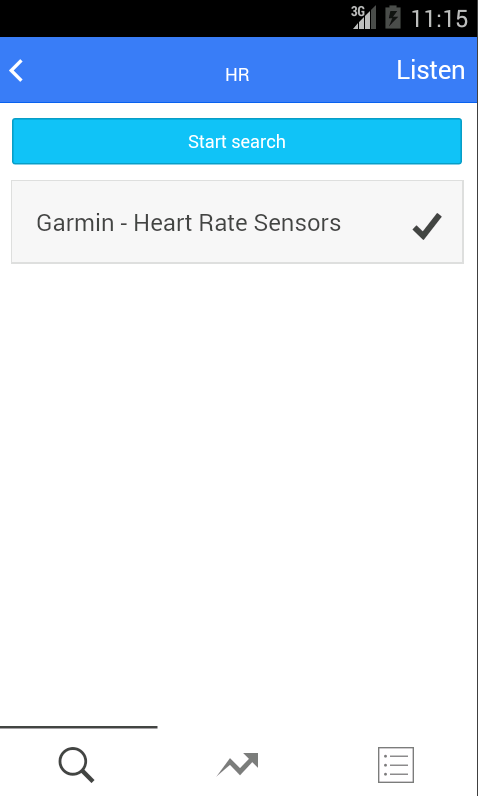
\includegraphics[width = 4cm, height=6.0cm]{Materials/Capture.PNG}\label{fig:capture_a}}
\hspace{10pt}\subfloat[Current heart rate]{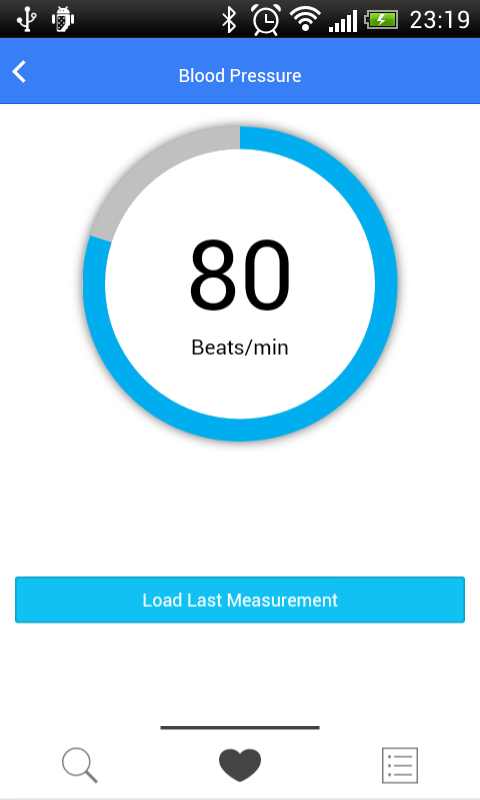
\includegraphics[width = 4cm, height=6.0cm]{Materials/Capture3.PNG}\label{fig:capture_b}}
\hspace{10pt}\subfloat[Long term heart rate]{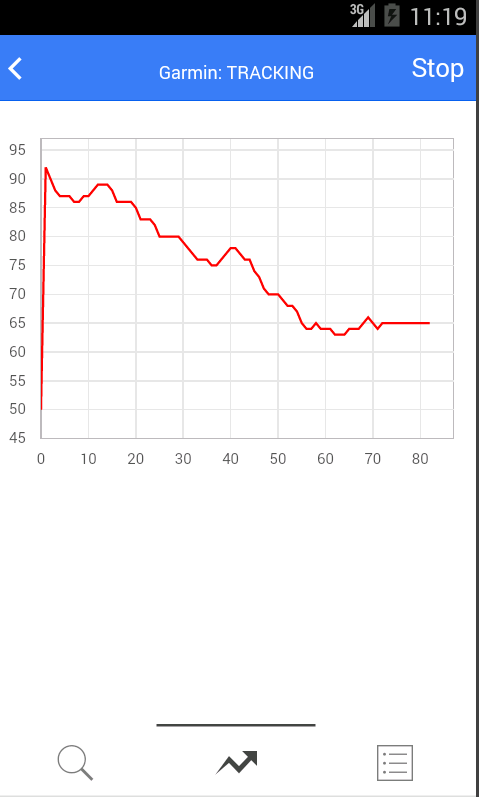
\includegraphics[width = 4cm, height=6.0cm]{Materials/Capture2.PNG}\label{fig:capture_c}}
\end{tabular}
% figure caption is below the figure
\caption{Mobile Application Preview}
\label{fig:mob_app_prev}
\end{figure*}   

\subsection{Integration with EEGBase}

When data are collected they are stored on the device SD card. Data can be visualized directly on mobile phone screen or they can be transfered to the server. Data on the server are stored for future processing. The main functionalities of EEGBase include storing, uploading, downloading, and managing experimental data and metadata. Currently we are implementing an advanced system of user templates for different kind of metadata. These templates are also stored in the odML format. The template system is also used for data from the sensors. 

More specifically odML is  a free form tree-like structure of sections, properties and values. It enables us to easy define a different kind of metadata for various experiments. Such a template can be defined according to different data coming from different sensors. If we store e. g. data from a blood pressure sensor we  defined a section \emph{blood\_presure} with several properties: \textit{systolic\_pressure}, \textit{diastolic\_pressure}, \textit{mean\_pressure}, \textit{heart\_rate}. Listing \ref{odml_example} shows a JSON representation of proposed data structure. The document is simplified to keep readability. A complete document contains a complete set of properties describing the experiment.

Technically EEGBase provide a RESTful API with methods for obtaining user's experiments and uploading newly collected data. The user can select an automatic data upload triggered once the user gets on-line or he/she can enforce the upload manually. The data on the server side are transferred to an odML document that is stored in the Elasticsearch noSQL database. The data are visualized on the server as shown in Figure \ref{fig:EEGBase}.


\begin{figure}
  %\vspace{-0.2cm}

  \centering
   {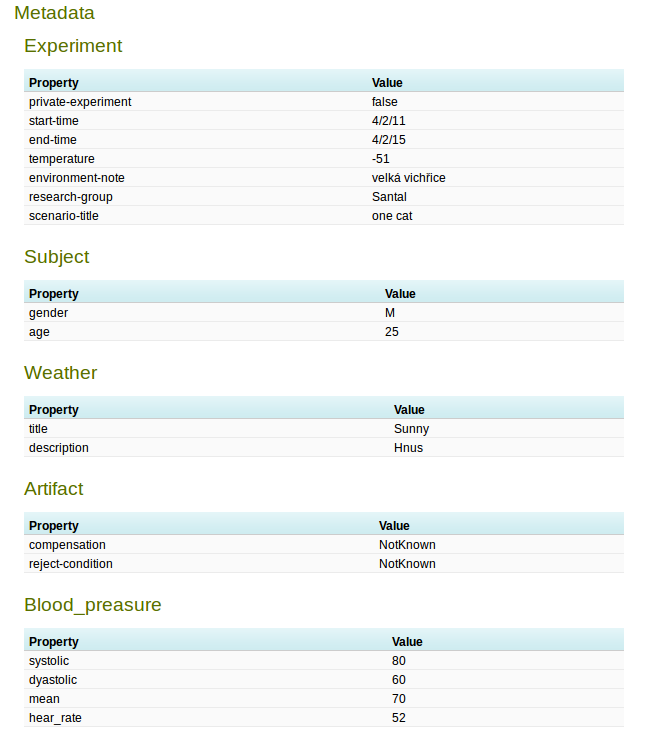
\epsfig{file = Materials/portal_example2.png, width = 8cm}}
  \caption{Data stored in EEGBase}
  \label{fig:EEGBase}
 \end{figure}


\begin{lstlisting}[language=json,caption=blood preasure examle, label=odml_example]
{
   "_index":"eegdatabase",
   "_type":"experiment",
   "_id":"167",
   "_source":{
      "experimentId":"167",
      "params":[
      ],
      "userId":243,
      "groupId":18,
      "metadata":{
         "odML":{
            "date":"2015-07-03",
            "xmlns:gui":"http://www.g-node.org/guiml",
            "section":[
               {
                  "name":"blood_pressure",
                  "property":[
                     {
                        "name":"systolic",
                        "value":{
                           "type":"int",
                           "content":80
                        },
                     },
                     {
                        "name":"dyastolic",
                        "value":{
                           "type":"int",
                           "content":60
                        },
                     },
                        "name":"mean",
                        "value":{
                           "type":"int",
                           "content":70
                        },
                     },
                     {
                        "name":"heart_rate",
                        "value":{
                           "type":"int",
                           "content":52
                        },
                     },
                  ],
                  "type":"blood_preasure"
               }
            ],
            "version":1
         }       
      }   
   } 
}
\end{lstlisting}


\section{\uppercase{Future Work}}
\label{future-work}
\noindent
Because the presented system serves only as a proof-of-concept implementation that supports only limited set of sensors. The main emphasis has been on the proposal of a universal open format for expressing the sensors data. The format defines the structure and the terminology for sensors supported in the system. Our future work includes the extension of this terminology to cover a widest collection of health sensors. When this terminology is designed we will extend the mobile app to convert data transfered in Bluetooth or ANT+ profiles to an odML document satisfies this terminology. Such a described data can be fully managed in systems such as EEGBase. A new release of EEGBase with the support of the presented terminology is also our future work. When this work is done we will release a complete description of designed terminology. This terminology can serve to developers of similar systems. The mobile system will be also extended to support widest collection of sensors.




\section{\uppercase{Conclusions}}
\label{sec:conclusion}

\noindent 
We observed that there is a diverse collection of available sensors on the market. These sensors vary in used data format, topology of data transfer or a transfer protocol. When the data are to be processed they must be collected and stored in databases. We identified topologies distinguishing sensors according to a way of management with data and selected the three layers topology as the most suitable for their long-term storage and processing. Because of the sensors producers use own systems and proprietary data formats they are read, transfered and processed with difficulties. As a solution we presented a prototype of a custom terminology used for expressing data from sensors. This terminology is implemented in the Android system. A limited set of sensors is supported in this implementation. A complete process from collecting data by the mobile system, its storage in a universal format respecting presented ontology, and their storage in EEGBase is outlined. This innovative approach can serve as a standard for developers of neuroinformatics databases when they want to collect data from health sensors. Respecting ANT+ or Bluetooth profiles by sensors producers is only one limited factor.

\section*{\uppercase{Acknowledgements}}

\noindent 
Will be added in CR version


\vfill
\bibliographystyle{apalike}
{\small
\bibliography{citations-healthinf-2016,frontiers,bibliography,neuroportals}


\vfill
\end{document}

